

%\begin{document}

	
	RFID, \textit{Radio Frequency Identification}, é uma tecnologia que está em crescente uso e evolução, devido às suas possíveis aplicações e os benefícios que sua utilização propiciam. Seu principal uso é no monitoramento de ativos, permitindo conhecer toda a trajetória de um produto, desde o início da cadeia produtiva até o consumidor final. 
	
	Avanços tecnológicos na fabricação de semicondutores permitiram tanto a redução do custo quanto a do tamanho dos componentes. Antes, as tags eram do tamanho de um forno-microondas e os leitores construídos com antenas gigantescas. Hoje em dia, podemos encontrar leitores do tamanho de um moeda, e tags do tamanho de um grão de arroz, alavancando ainda mais a adoção da tecnologia RFID. Qualquer sistema de identificação no qual um dispostivo eletrônico usa radio frequência para o variações no campo magnético para comunicar e está anexado a um item, é definido como um RFID.
	
	Os dois principais componentes deste tipo de sistema são a \textit{Tag}, a qual é o dispositivo de identificação anexado ao item que desejamos monitorar, e o \textit{Leitor}, que é o dispositivo responsável por reconhecer as Tags e ler as informações contidas nelas. O leitor pode então informar outros sistemas sobre a presença das tags, através de um \textit{RFID Middleware}. Este é uma ferramenta que fornece a interface entre os leitores e o restante do sistema de informação. Na figura a seguir, podemos ver o sistema em questão:
	
	\begin{figure}[h!]
		\centering
		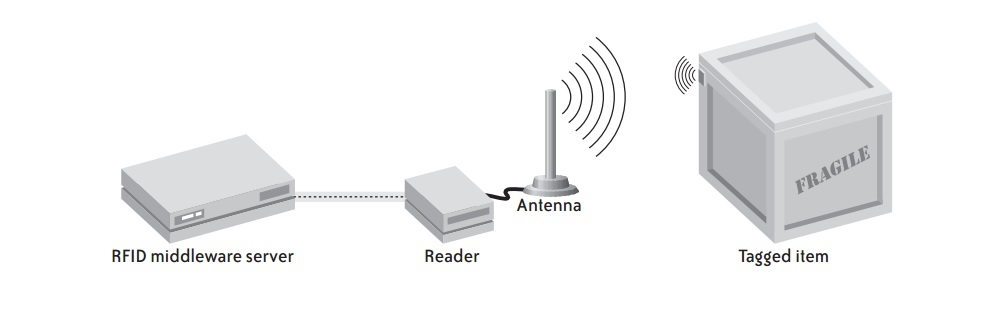
\includegraphics[width=0.6\linewidth]{rfidsys2}
		\caption{Sistema RFID típico, retirado de \cite{rfidbook}}
		\label{fig:rfidsys}
	\end{figure}
	
	Alguns dos benefícios do RFID são resumidos abaixo:
	\begin{itemize}
		\item Não há necessidade de alinhamento dos itens para leitura;
		\item Alta velocidade de inventário, pois vários itens podem ser lidos simultaneamente;
		\item Capacidade de identificar unicamente bilhões de itens;
		\item Variedade na forma das tags;
		\item Reusabilidade de tags.
	\end{itemize}
	
	\subsection{Evolução na adoção do RFID}
	De acordo com \cite{rfidbook}, podemos dividir o progresso de adoção do RFID em 5 períodos: \textit{Proprietary era}, \textit{Compliance era}, \textit{RFID-enable Enterprise era}, \textit{RFID-enable Industies era} e \textit{Internet of Things era}(Figura \ref{fig:rfideras}).
	
	\begin{figure}[h!]
		\centering
		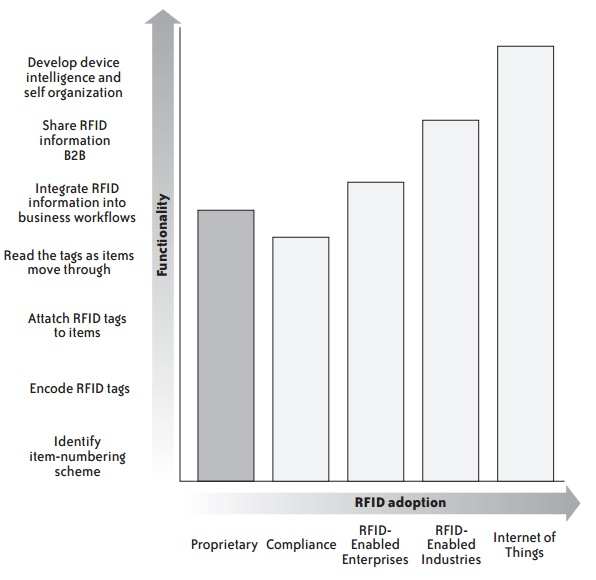
\includegraphics[width=0.6\linewidth]{rfideras}
		\caption{Evolução do RFID, retirado de \cite{rfidbook}}
		\label{fig:rfideras}
	\end{figure}
	
	No início (\textit{Proprietary era}), o RFID era usado para monitorar tipos particulares de itens e esta informação permanecia dentro das organizações que utilizavam o sistema. Isso fazia com que os sistemas fosse bastante específicos, dificultando bastante a comunicação entre parceiros de negócios. Alguns dos itens monitorados eram carros de trem, chassis de automóveis e gado leiteiro. Nesta época as tags ainda eram caras, logo estas eram reutilizadas sempre que possível. 
	
	Na \textit{Compliance era}, que representa o período atual, as empresas utilizam o RFID principalmente para garantir a interoperabilidade entre parceiros de negócios e agências regulatórias, não usando frequentemente os dados RFID para, por exemplo, aperfeiçoar alguns processos e melhorar a produtividade. A escassez de padrões e a falta de confiabilidade das novas tecnologias, impedem que as tags funcionem tão bem na prática como na época anterior.
	
	No futuro, teremos a \textit{RFID-Enabled Enterprise era}, na qual as empresas começarão a utilizar as informações coletadas do RFID para o aprimoramento dos próprios processos. Isso será alcançado com a estabilização dos padrões e queda significativa dos custos. As empresas passarão a monitorar itens individuais ao invés de unidades de transporte, permitindo a coleta de mais informações sobre o processo. Entretanto, mesmo com a larga adoção interna do RFID, as empresas ainda precisam desenvolver os padrões necessários para permitir a troca de informações com os parceiros de negócios. 
	
	Em seguida teremos a \textit{The RFID-Enabled Industries era}, onde o uso de padrões RFID, redes de informação RFID, acordos de negócios e políticas de segurança e privacidade permitirão que empresas e cadeias de suprimentos troquem dados de forma segura e confiável entre si. Isso permitirá a descoberta de novas informações através do estudo  do grande volume de dados que estará disponível.   
	   
	Por fim, teremos a \textit{The Internet of Things era} que é atualmente uma previsão, na qual a ubiquidade da tecnologia RFID mudará a forma como vemos a relação entre informação, objetos físicos e localização. Por exemplo, a geladeira de nossa casa estará conectada à Internet e será capaz de ler a data de validade dos alimentos presentes e nos informar se algum deles já venceu. Além disso, ela poderá checar se algum produto está faltando e automaticamente realizar o pedido deste junto ao supermercado.
	
	A forma e velocidade com que os diversos tipos de usuários passarão por essas épocas não será feita de maneira uniforme. Atualmente, existem usuários que ainda estão na \textit{Proprietary era}, enquanto outros já estão começando a aplicar os conceitos da \textit{RFID-enabled Industries e Internet of Things}. Em algumas áreas, o RFID ainda nem começou a ser implementado.
	
	
	\subsection{Sistemas RFID}
	
	Em um sistema RFID, destacam-se os seguintes componentes: Tags, Leitores e Middleware. Todos podem ser vistos na figura \ref{fig:rfidcomp} e serão explicados com mais detalhes em seguida.
	
	\begin{figure}[h!]
		\centering
		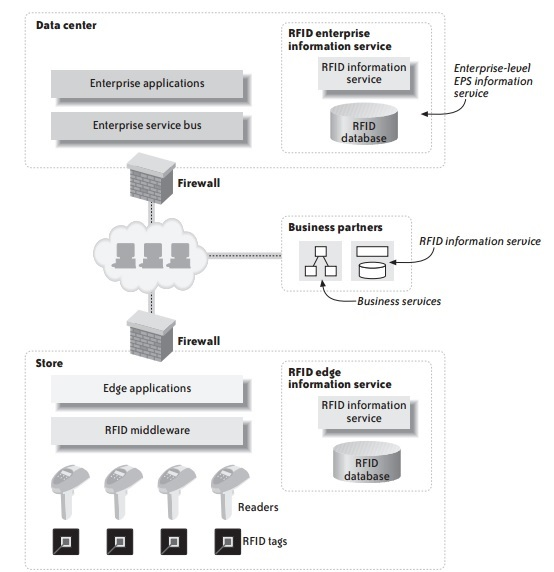
\includegraphics[width=0.5\linewidth]{rfidsys3}
		\caption{Componentes de um sistema RFID, retirado de \cite{rfidbook}}
		\label{fig:rfidcomp}
	\end{figure}
	
	\subsubsection{Tags}
	São elementos fisicamente acoplados a um objeto, possuindo uma memória para armazenamento de dados. Toda tag RFID possui algum tipo de bobina ou antena, de forma a permitir sua leitura, e precisa ter as seguintes funcionalidades:
	
		\begin{itemize}
			\item Toda tag tem que ser anexada a um item
			\item Toda tag tem que ser capaz de se comunicar usando radiofrequência
		\end{itemize}
	

	 Existem tags de diversos tamanhos e formatos, nos dando a flexibilidade de escolher a que melhor se encaixará na aplicação a ser desenvolvida (figura \ref{fig:rfidtags}). Elas podem ser passivas, ativas ou semi-passivas. As passivas obtém sua energia dos leitores. Já as ativas possuem uma bateria interna para fornecer a energia necessária para o processamento de suas tarefas.	
	 As tags semi-passivas são capazes de obter eneergia dos leitores e também possuem uma bateria interna.
	 
		\begin{figure}[h!]
			\centering
			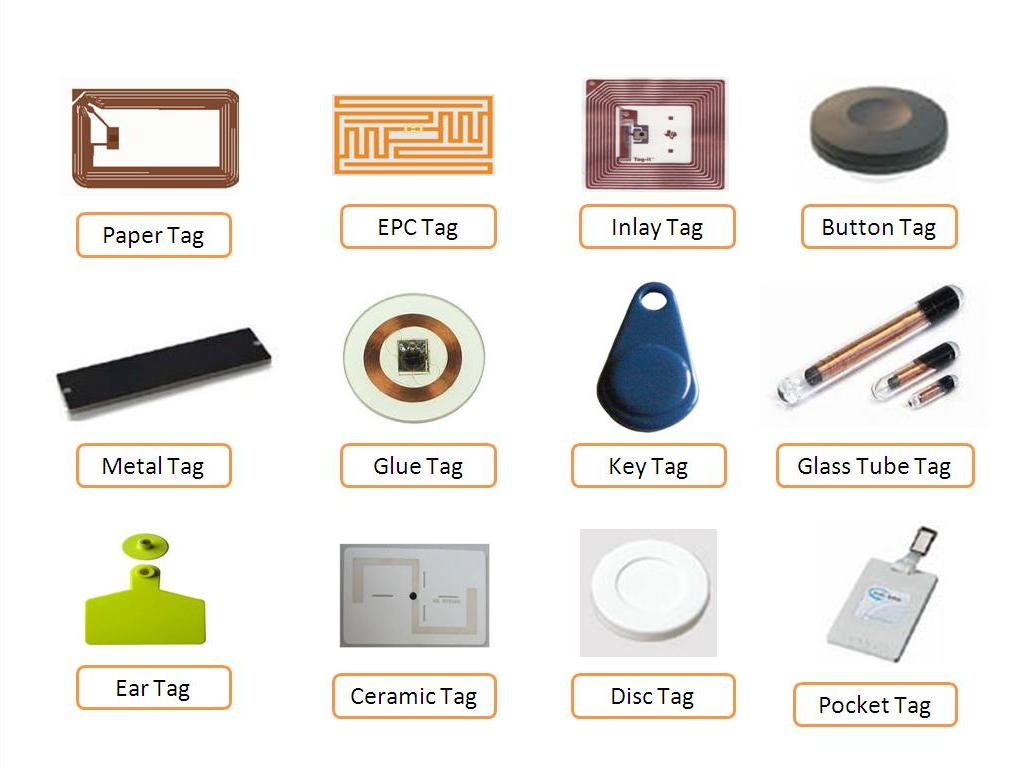
\includegraphics[width=0.5\linewidth]{rfidtagas}
			\caption{Alguns modelos de tags disponíveis}
			\label{fig:rfidtags}
		\end{figure}
	
	Como a comunicação é feita por radiofrequência, precisamos levar em consideração o meio de transmissão da informação, que neste caso é o ar. Portanto, devemos levar em consideração os seguintes atributos, os quais definem a interface do ar:   
	
	\paragraph{Modo de comunicação} Dividido em \textit{full-duplex} (FDX)/\textit{half-duplex} (HDX) ou \textit{Sequencial} (SEQ). Sistemas FDX ou HDX difundem a informação vinda das tags quando acionamos o leitor. Já nos sistemas SEQ é implementado um acionamento periódico do leitor, no qual ele fica desligado enquanto a tag está respondendo.	
	\paragraph{Frequência de Operação} A frequência de operação especifica o intervalo de frequências em que será feita a comunicação, resolvemos problemas relacionados a interferência entre os aparelhos. A tabela \ref{tab:freqapp} mostra a relação entre os possíveis intervalos operação e as respectivas aplicações.

		\begin{table}
			\centering
			
			\begin{tabular}{|c|c|p{9cm}|}
				
				\hline Nome & Intervalo de frequências & Aplicações \\ 
				\hline LF & 30-300 kHz & Identificação de animais e leituras próximas de itens cheios de água \\ 
				\hline HF & 3 - 30 MHz & Controle de acesso a edifícios \\ 
				\hline UHF & 300 MHz - 3 GHz & Caixas e paletes \\ 
				\hline Microondas & $>$ 3 GHz & Identificação de veículos em geral \\ 
				\hline 
				
			\end{tabular} 	
			\caption{Frequência de operação e suas aplicações}
			\label{tab:freqapp}
		\end{table}	

	\paragraph{Tipos de Chaves} O tipo de chave define os atributos da portadora que tranportará o sinal, selecionando o tipo de modulação que deverá ser usada.
	
	\paragraph{Codificação} A codificação determina como a tag e o leitor interpretam a informação sendo transmitida pela portadora, ou seja, são responsáveis pela demodulação.
  
	\paragraph{Acoplamento} O acoplamento determina como o circuito do leitor influencia o da Tag, e vice-versa, afetando a distância com que eles precisarão estar entre si para haver a troca de dados.\\
	 
	Devemos também levar em consideração a forma com que as tags armazenam e processam as informações. A capacidade de aramzenamento vai de 1 bit até kilobytes de dados. Os tipos mais comuns são:
	
	\paragraph{EAS - Electronic Article Surveillance} São tags usando principalmente para a prevenção de roubo. Possuem somente 1-bit, podendo indicar somente a presença ou não de uma tag, por exemplo. São sempre passivas e geralmente não possuem microchips e memória para armazenamento de dados, sendo simples e baratas. 
	
	\paragraph{SAW - Surface Acoustic Waves} Operam no intervalo das microondas, não possuem processadores e sua capacidade é de até 32-bits. Funcionam a partir do seguinte princípio: O leitor emite ondas de rádio, que são convertidas em uma onda acústica na superfície do chip SAW. Essa onda acústica se propaga pela tag, passando por uma série de refletores, produzindo pulsos acústicos de onda unicamente condificados. Esse pulsos são convertidos novamente  para ondas de rádio e tramitidos através de reflexão para o leitor.
	
		\begin{figure}[h!]
			\centering
			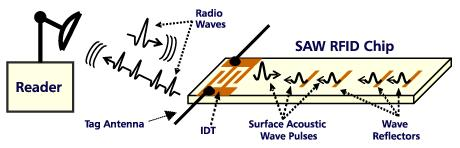
\includegraphics[width=0.5\linewidth]{sawrfid_chip}
			\caption{Funcionamento das tags SAW}
			\label{fig:sawtag}
		\end{figure}
		
	Algumas tags apresentam um comportamento mais complexo, possuindo máquinas de estado incorporadas em chips customizados, permitindo que elas exerçam um papel mais ativo no sistema. Por causa disso, são geralmente mais caras. 
	
	\subsubsection{Leitores}
	Os leitores RFID são os componentes responsáveis pela leitura das tags, geração de evnetos e finalmente envio dos dados à camada de \textit{Middleware}. Os elementos físicos básicos de um leitor são: antena, controlador e interface de rede.
	
	A \textbf{antena} é o elemento principal da comunicação, cujo papel é enviar e receber as informações na forma de ondas de radio-frequência. Dependendo da aplicação, um leitor pode ter mais de uma antena. O \textbf{controlador} tem como função executar os protocolos de comunicação e controlar o transmissor. Pode ser implementado em um chip ou até em sistemas maiores e mais robustos, como microcomputadores. A \textbf{interface de rede} é essencial para a comunicação com a camada de middleware e também com outros dispositivos. As formas mais comuns de se fazer isto pe usando as interfaces RS 232, Ethernet, Bluetooth e ZigBee.
	
	Um leitor RFID também pode ser divido em 4 partes lógicas e abstratas, como pode ser vista na figura \ref{fig:reader}. 
		
		\begin{figure}[h!]
			\centering
			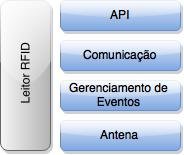
\includegraphics[width=0.25\linewidth]{reader}
			\caption{Componentes lógicos de um leitor RFID. Adaptado de \cite{rfidbook}}
			\label{fig:reader}
		\end{figure}
	
	\paragraph{API} Fornece uma interface de programação que possibilita outras aplicações requisitar inventários de tags, monitorar a vida útil e configurar o leitor. Sua principal função é criar mensagens para a camada de Middleware a partir dos dados lidos e interpretar as recebidas.
	
	\paragraph{Comunicação} Gerencia os detalhes técnicos relativos aos protocolos usados na troca de dados com o Middleware.
	
	\paragraph{Gerenciamento de Eventos} Define quais eventos de leitura são relevantes para serem disponibiliados ao Middleware. Tem papel importante na redução de tráfego na rede, pois impedem que eventos irrelevantes sejam transmitidos com frequência.
	
	\paragraph{Antena} Consiste na interface e lógica que permite aos leitores interrogar as tags sobre seu estado atual e controlar as antenas físicas. Implementa os protocolos de trocas de dados usando rádio-frequência bem como a eletrônica da interface com o ar.

	
	\subsubsection{Middleware RFID}
	
	O middleware RFID é um software que intermedia a comunicação entre o sistema de informação da organização (MES, ERP) e a infraestrutura de hardware do sistema RFID (tags,leitores acoplados à rede). Sua função é coletar, filtrar e agregar os dados provenientes dos leitores \cite{renatarfid}. \\
	Portanto, podemos inferir uma estrutura básica para o middleware composta de 3 componentes lógicos, como pode ser visto na figura \ref{fig:middleware}.
		
		\begin{figure}[h!]
			\centering
			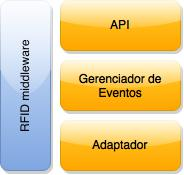
\includegraphics[width=0.25\linewidth]{middleware}
			\caption{Componentes lógicos do middleware. Adaptado de \cite{rfidbook}}
			\label{fig:middleware}
		\end{figure}
	
	\paragraph{API} Sua função principal é fornecer um mecanismo padrão com o qual as aplicações podem se registrar e receber dados vindos dos leitores RFID. Ela também deve fornecer uma API para a configuração, monitoramento e gerenciamento do middleware e os letiroes e sensores controlados por ele.
	\paragraph{Gerenciador de eventos} Em aplicações de grande porte, o volume de informação coletados dos leitores RFID é muito grande, tornando imprático que se salve todos os dados. Portanto, o papel do gerenciador de eventos é agregar, consolidar e filtrar esses dadods, de forma a enviar somente as informações mais relevantes aos sistemas gerenciais.
	\paragraph{Adaptador} Atualmente existem dezenas de fabricantes de leitores RFID, os quais fornecem interfaces diferentes para uso de seus produtos. Portanto, é papel do adaptator fornecer uma interface de alto-nível que implemente os protocolos proprietários, fazendo com que os usuário não precisem se preocupar com estes detalhes. Isso reduz significativamente as dificuldades na integração dos dados RFID.
	
	A figura \ref{fig:midarc} apresenta um modelo conceitual para a implementação real de um middlware RFID. Nele podemos ver o papel e a importância dos componentes lógicos exibidos anteriormente, e como o middleware pode fornecer interfaces que permitem a integração com sistemas JAVA e .NET, por exemplo.
	
		\begin{figure}[h!]
			\centering
			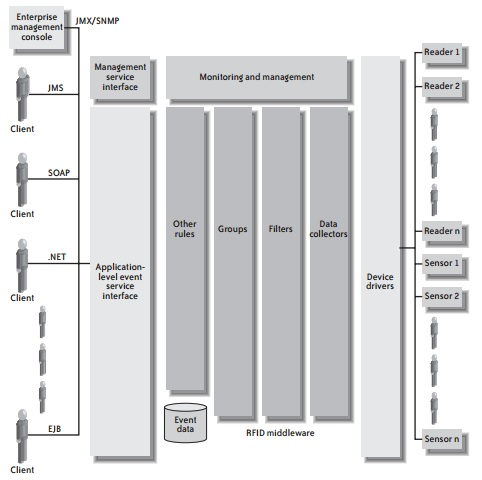
\includegraphics[width=0.5\linewidth]{midarc}
			\caption{Arquitetura conceitual de um Middleware RFID. Retirado de \cite{rfidbook}}
			\label{fig:midarc}
		\end{figure}
	
	\subsection{Aplicações}
	Devido às características discutidas anteriormente, podemos concluir que existirá uma variedade enorme de aplicações da tecnologia RFID. De acordo com \cite{rfidbook}, a maioria delas podem ser classificadas nos seguintes grupos:
	\begin{itemize}
		\item Controle de acesso
		\item Tag and Ship funcionamento do sistema.
		\item Localizar paletes e caixas
		\item Localizar e monitorar
		\item Prateleira inteligente
	\end{itemize}
	
	Nas próximas seções deste trabalho serão expostos alguns estudos de caso exemplificando algumas aplicações prática. A partir destes exemplos será possível entender melhor como funcionam na prática os diversos componentes de um sistema RFID. A ultima seção descreverá o EPCGlobal, que é um padrão importante adotado empresas de peso, cuja utilização está em crescente uso devido aos benefícios propiciados pela sua adoção em aplicações de \textit{Supply Chain Management}.
%	\newpage
%	 \bibliographystyle{plain}
%	 \nocite{*}
%	 \bibliography{biblio_doc}
	 


%\end{document} 